\section{Probability distributions}

\subsection{Normal}

\subsection{Chi-squared}

\marginnote{
Let $z_i \stackrel{iid}{\sim} \mathcal{N}(0,1)$.
Then $Q$ follows the chi-squared distribution with $k$ degrees of freedom
if it can be written as
\[
Q = z_1^2 + z_2^2 + \ldots + z_k^2.
\]

This definition is a particular case of the geometric one.
Consider projecting a vector $z = (z_1, z_2, \ldots, z_n)$ form $\mathbb{R}^n$
onto the~$k$-dimensional subspace $S$ of vectors which first $k$ coordinates
are arbitrary and all the rest are zeros. As a result we would get
\[
\hat z = (z_1, z_2, \ldots, z_k, 0, \ldots, 0).
\]
Squaring the length of the projection, we obtain
\[
Q = \lVert \hat z \rVert = z_1^2 + z_2^2 + \ldots + z_k^2.
\]
}

\begin{theorem}
Consider a random vector $z \in \mathbb{R}^n$ which components are independent
and follow standard normal distribution, $z_i \sim \mathcal{N}(0,1)$.
Consider also a fixed $k$-dimensional subspace $L$ in $\mathbb{R}^n$.
Let the projection of vector $z$ onto the subspace $L$ be $\hat z$ and
its length squared $Q$
\[
Q = \lVert \hat z \rVert^2 = \langle \hat z, \hat z \rangle = \hat z^T \hat z
\]
Then $Q$ follows the chi-squared distribution with $k$ degrees of freedom.
\end{theorem}

\begin{proof}
First, it can be shown that the~projected vector $\hat z$ is the~original vector $z$
multiplied by the~projection matrix $H = X(X^T X)^{-1}X^T$ where the columns of $X$
are fixed linearly independent vectors $x_1, \ldots, x_k$ in $L$
or equivalently $colX = Lin(x_1, \ldots, x_k)$.
This matrix is  also often referred to as `hat-matrix'.
Then the statement in~the~theorem can be rewritten as follows:
\[
\hat z^T \hat z = (Hz)^T Hz = z^T H^T H z = z^T H^2 z = z^T H z,
\]
applying the idempotence property in the last step.

Another nice property of~the~hat-mattix is symmetry.
Thus, it can be decomposed as
\[
H = P D P^T,
\]
where we choose the vectors of matrix $P$ to be unit and orthogonal,
and $D = diag{\lambda}$ where $\lambda_i$ is an eigenvalue of $H$.

\begin{marginfigure}
  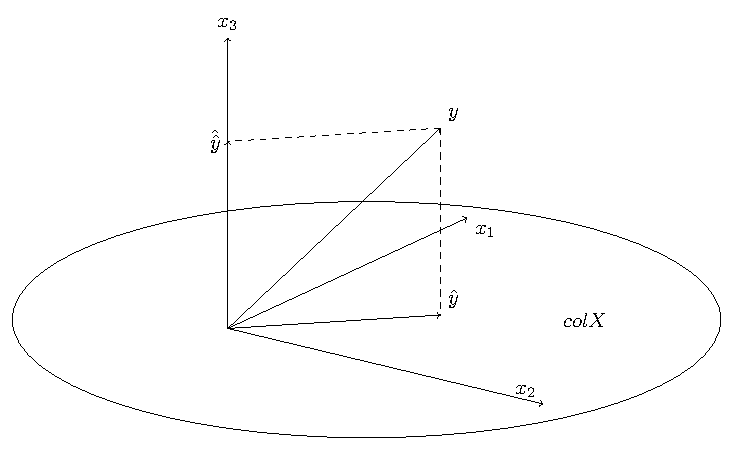
\includegraphics[width=\linewidth]{figures/04_chi_squared_example.pdf}
  \caption{Consider a $3$-dimensional example, $colX = Lin(x_1, x_2)$ and $col^{\perp}X = Lin(x_3)$.
  $H x_1 = x_1$ and $H x_2 = x_2$ since they are in $colX$. However, $H x_3 = 0$ as $x_3 \perp colX$.
  Projecting an arbitrary vector onto $colX$ yileds $Hy = \hat y \in Lin(x_1, x_2)$
  while projecting onto $col^{\perp}X$ results in $(I-H)y = \hat{\hat y} \in Lin(x_3)$.}
\end{marginfigure}

Since $H^2 = H$ the eigenvalues are either $0$ or $1$.
Recall that $H$ projects a vector onto $colX$.
Then for any $x_i$, $i = 1, \ldots, k$, $H x_i = x_i \cdot 1$ since
any $x_i$ is already in $colX$. This implies that $\lambda_1 = \ldots = \lambda_k = 1$.
There are also $n-k$ vectors in the subspace orthogonal to $colX$.
So for any $x_i$, $i= k+1, \ldots, n$, the orthogonal projection yields zero.
We conclude that $\lambda_{k+1} = \ldots = \lambda_n = 0$.

Rewritting the theroem statement further, we obtain
\[
z^T H z = z^T P D P^T z = (P^T z)^T D (P^T z) = \tilde z^T D \tilde z = \tilde z_1^2 + \ldots + \tilde z_k^2.
\]
Now we explore $\tilde z$ given $z \sim \mathcal{N}(0, I)$:
\begin{align*}
&\tilde z = P^T z \\
&\E(\tilde z) = \E(P^T z) = P^T \E(z) = 0 \\
&\Var(\tilde z) = \Var(P^T z) = P^T \Var(z) (P^T)^T = P^T P = I
\end{align*}
So we conclude that $\tilde z_1^2 + \ldots + \tilde z_k^2 \sim \chi^2_k$.




\end{proof}




\subsection{Student's}

\subsection{t-test}

In a simple linear regression model
\[
y = \beta_1 + \beta_2 x + \varepsilon
\]
the adjusted t-value $\frac{t}{\sqrt{n-2}}$ when $H_0: \beta_2 = 0$ is tested
can be expreesed in terms of the angle between $y$ and $\hat y$ $\varphi$ and
is equal to $\ctg \varphi$.

Recall that the t-statistic is defined in the following way:
\[
t = \frac{\hat \beta - \beta}{s.e.(\hat\beta)}
\]
Adjusting this formula for the null hypothesis $H_0: \beta_2 = 0$, we obtain
\begin{equation}\label{eq:tstat}
t = \frac{\hat \beta_2}{s.e.(\hat\beta_2)}
\end{equation}
Then, we need to express $s.e.(\hat\beta_2)$ in terms of vectors which can be
plotted. From standard OLS procedure it follows that
\begin{equation}\label{eq:varbeta2}
\Var(\hat \beta_2) = \frac{\sigma}{\sum_{i=1}^n (x_i - \bar x)^2}
\end{equation}
Since actual $\sigma$ is unknown the estimator will be used instead:
\begin{equation}\label{eq:sigmaest}
\hat \sigma^2 = \frac{RSS}{n-2}
\end{equation}
Substituting \eqref{eq:varbeta2} and \eqref{eq:sigmaest} into \eqref{eq:tstat}
divided by $\sqrt{n-2}$, we obtain
\begin{align*}
\frac{t}{\sqrt{n-2}} &= \frac{\hat \beta_2}{\sqrt{n-2}\widehat{s.e.}(\hat\beta_2)} \\
&= \frac{\hat \beta_2}{\sqrt{n-2}\frac{\hat \sigma}{\sqrt{\sum_{i=1}^n (x_i - \bar x)^2}}} \\
&= \frac{\hat \beta_2 \sqrt{\sum_{i=1}^n (x_i - \bar x)^2}}{\sqrt{n-2}\frac{\sqrt{\sum_{i=1}^n (y_i - \hat y_i)^2}}{\sqrt{n-2}}} \\
&= \frac{\hat \beta_2 \vert x^c \vert}{\sqrt{RSS}}
\end{align*}
where $ \vert x^c \vert = \sqrt{\sum_{i=1}^n (x_i - \bar x)^2}$ is the length of the
centred vector $x$.

Now the result can be demonstrated visually.
Again we will project $x$ and $y$ vectors onto the $Lin^{\perp}(\mathbf{1})$ so as to
get their centred versions $x^c$ and $y^c$.
Then, we perform regression of $y$ onto $Lin(x, \mathbf{1})$ which results in $\hat y$.
Following that, we project $\hat y = \hat \beta_1 + \hat \beta_2 x$ onto $Lin^{\perp}(\mathbf{1})$
which yields $\hat \beta_2 x^c$.
After all, we translate $\sqrt{RSS}$ onto $Lin^{\perp}(\mathbf{1})$.
These steps are demonstrated in Figure~\ref{fig:ttest_3d}.

Looking at Figure~\ref{fig:ttest_lin} which depicts the $Lin^{\perp}(\mathbf{1})$,
we derive
\[
\ctg \varphi = \frac{\hat \beta_2 \vert x^c \vert}{\sqrt{RSS}} = t
\]

\begin{figure}[ht!]
\begin{center}
\subfigure[]{
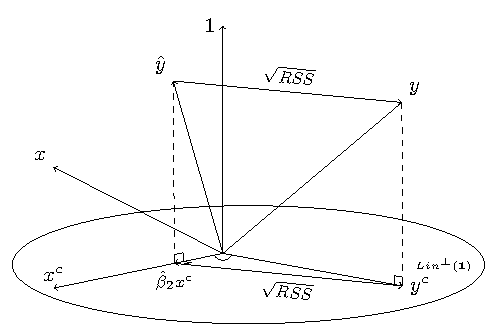
\includegraphics[width=0.45\linewidth]{figures/04_ttest.pdf}
\label{fig:ttest_3d}}
%\hspace{4ex}
\subfigure[]{
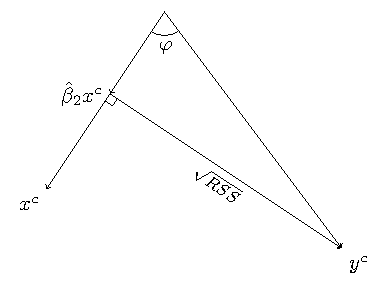
\includegraphics[width=0.45\linewidth]{figures/04_ttest_lin.pdf}
\label{fig:ttest_lin}}
\caption{\subref{fig:pcorr_t_x}: Regression of $y$ onto $Lin(x, \mathbf{1})$ and appropriate projections;
\subref{fig:pcorr_t_y}: $Lin^{\perp}(\mathbf{1})$.}
\end{center}
\end{figure}

\subsection{F-distribution}

\subsection{F-test}

The significance of several coefficients at once can be tested with the F-test.
The F-statistic has the following form
\[
F = \frac{(RSS_{R} - RSS_{UR})/q}{RSS_{UR}/(n-k_{UR})}
\]
where indices $R$ and $UR$ stand for the restricted and unrestricted models
respectively, $n$ — number of observations, $k$ — number of regressors,
$q$ — number of equtions used in the null hypothesis.

Due to plotting limitations, we consider the unrestricted model to be
\[
y = \beta_1 + \beta_2 x + u
\]
and the restricted model to be
\[
y = \alpha_1 + v
\]
Note that there was a choice in the restricted models.

We perform both regressions in order to get the ressiduals and plot them
in Figure~\ref{fig:ftest}.
Adjusted to the degrees of freedom, the ratio can be expressed in terms of the
angle between two vectors, $\varphi$, as demonstrated in Figure~\ref{fig:ftest}
\[
F = \frac{(RSS_{R} - RSS_{UR})/q}{RSS_{UR}/(n-k_{UR})} = \ctg^2 \varphi
\]

\begin{figure}
\centering
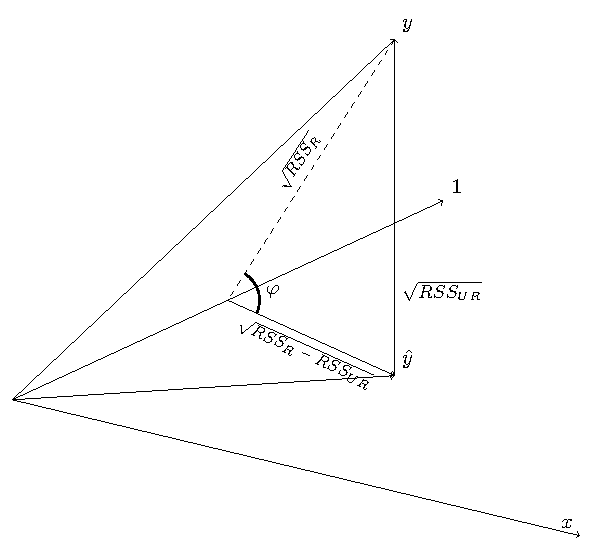
\includegraphics[width=0.55\linewidth]{figures/04_ftest.pdf}
\caption{F-statistic as the cotangens squared of $\varphi$}
\label{fig:ftest}
\end{figure}
